% !TEX TS-program = XeLaTeX

% Template for homework and assignments  
% Created by Mahmood Amintoosi, HSU
% Modified by Morteza Zakeri, IUST
% Last modified date:	13981110

\documentclass[12pt]{exam}
\usepackage[margin=20mm]{geometry}
\usepackage{verbatim}
\usepackage{lmodern} 
\usepackage{lipsum}
\usepackage{marginnote}
\usepackage[T1]{fontenc}
% در ورژن جدید زی‌پرشین برای تایپ متن‌های ریاضی، این سه بسته، حتماً باید فراخوانی شود
\usepackage{amsthm, amssymb, amsmath}
\usepackage{relsize} % for \mathlarger

\usepackage{setspace}
\usepackage{enumerate}
\usepackage{enumitem}
\usepackage{xcolor}

%\usepackage{hyperref}
\usepackage{bookmark}
\usepackage{hyperref}

\usepackage[final]{graphicx}
\graphicspath{{./figs/}}
\usepackage{tikz}

\usepackage{caption}
\usepackage{multirow}
%\usepackage[table,xcdraw]{xcolor}
\usepackage{listing}
\usepackage[final]{listings}

\usepackage{blindtext}
\usepackage[most]{tcolorbox}
\newtcolorbox{mybox}[2][]{boxrule=0pt, width=\textwidth, arc=0mm, colback=gray!10}
\newtcolorbox{mybox2}[2][]{width=\textwidth, colback={green}, colbacktitle=yellow, coltitle=blue, title=#2,#1}

\newtcolorbox{mybox3}[2][]{%
    width=\textwidth,
    arc=0mm,
   % boxrule=0pt,
    enhanced, 
    breakable,
    frame hidden,
    overlay broken = {
        \draw[line width=0.50mm, gray, rounded corners]
        (frame.north east) rectangle (frame.south west);},
}


\usepackage[framemethod=tikz]{mdframed} 
%\usepackage{ntheorem}

\newmdtheoremenv[
backgroundcolor=gray!10,
splittopskip=2\baselineskip,
middleextra={\node[anchor=north west,font=\bfseries,inner xsep=0pt,xshift=10pt] at (P-|O) {Example~\thetest\ (Continued)};},
secondextra={\node[anchor=north west,font=\bfseries,inner xsep=0pt,xshift=10pt] at (P-|O) {Example~\thetest\ (Continued)};}
]{mybox4}{Example}


%################################

\usetikzlibrary{lindenmayersystems}

\pgfdeclarelindenmayersystem{A}{
	\rule{F -> FF[+F][-F]}
}

\pgfdeclarelindenmayersystem{B}{
	\rule{F -> ffF[++FF][--FF]}
}

\pgfdeclarelindenmayersystem{C}{
	\symbol{G}{\pgflsystemdrawforward}
	\rule{F -> F[+F][-F]FG[+F][-F]FG}
}

\pgfdeclarelindenmayersystem{D}{
	\symbol{G}{\pgflsystemdrawforward}
	\symbol{H}{\pgflsystemdrawforward}
	\rule{F -> H[+HG][-HG]G}
	\rule{G -> HF}
}

\tikzset{
	type/.style={l-system={#1, axiom=F,order=3,step=4pt,angle=60},
		blue, opacity=0.4, line width=.5mm, line cap=round   
	},
}

\newcommand\drawsnowflake[2][scale=0.2]{
	\tikz[#1]
	\foreach \a in {0,60,...,300}  {
		\draw[rotate=\a,#2] l-system;
	};
}

%################################

%%%%%%%%%%%%%%%%%%%%%%%%%%%%%%%%%%%%%%%%%%%%%%%%%%
\usepackage{xepersian}
\settextfont[Path={./font/Niloofar/}, BoldFont={XBNiloofarBd.ttf}, ItalicFont={XBNiloofarIt.ttf}, BoldItalicFont={XBNiloofarBdIt.ttf}, Scale=1.0]{XBNiloofar.ttf}

\setlatintextfont[Scale=0.90]{Times New Roman}
% چنانچه می‌خواهید اعداد در فرمول‌ها، انگلیسی باشد، خط زیر را غیرفعال کنید
\setdigitfont[Path={./font/Zar/}, BoldFont={XBZarBd.ttf}, ItalicFont={XBZarIt.ttf}, BoldItalicFont={XBZarBdIt.ttf}, Scale=1.0]{XBZar.ttf}

% اگر می‌خواهید که اعداد با فونت یکان نمایش داده شوند خط بالا را غیر فعال کرده و خط زیر را فعال کنید.

%\setdigitfont[Path={./font/Yekan/}, BoldFont={XMYekanBd.ttf}, ItalicFont={XMYekanIt.ttf}, BoldItalicFont={XMYekanBdIt.ttf}, Scale=1.0]{XMYekan.ttf}%{Persian Modern}

% تعریف قلم‌های فارسی و انگلیسی اضافی برای استفاده در بعضی از قسمت‌های متن
\defpersianfont\yagut[Path={./font/Yagut/}, BoldFont={XBYagutBd.ttf}, ItalicFont={XBYagutIt.ttf}, BoldItalicFont={XBYagutBdIt.ttf}, Scale=1.0]{XBYagut.ttf}

\defpersianfont\titlefont[Path={./font/Titre/}, BoldFont={XBTitreShadow.ttf}, ItalicFont={XBTitreIt.ttf}, BoldItalicFont={XBTitreShadowIt.ttf}, Scale=1.0]{XBTitre.ttf}

\defpersianfont\iranic[Path={./font/Zar/XBZarOblique/}, BoldFont={XBZarObliqueBd.ttf}, Scale=1.10]{XBZarOblique.ttf}%Italic}%

\defpersianfont\nastaliq[Path={./font/IranNastaliq/}, Scale=1.50]{IranNastaliq.ttf}
%%%%%%%%%%%%%%%%%%%%%%%%%%%%%%%%%%%%%%%%%%%%%%%%%%
% تعریف محیط قضایا، تعاریف، گزاره‌ها و مثال‌‌ها
\theoremstyle{plain}
\newtheorem{theorem}{قضیه}
\newtheorem{lemma}{لم}
\newtheorem{proposition}{گزاره}
\theoremstyle{definition}
%\newtheorem{definition}{تعریف}

%\newmdtheoremenv{definition}{تعریف}
%\newtcbtheorem[no counter]{definition}{تعریف}{width=\textwidth,
\newtcbtheorem{definition}{تعریف}{width=\textwidth,
 enhanced,
 sharp corners,
attach boxed title to top right={
    yshifttext = -1mm},
colback=white,
colframe=blue!75!black,
boxed title style={
    sharp corners,
    size=small,
    colback=blue!75!black,
    colframe=blue!75!black}}{definition}

\newtheorem{example}{مثال}
\newtheorem{prob}{سوال}
\theoremstyle{remark}
\newtheorem{corollary}{نتیجه}
\newtheorem{remark}{ملاحظه}
% تعیین مشخصات فایل PDF
\hypersetup{
	pdftitle={تمرین سـری دوم درس نظریه بازی‌ها},
	pdfauthor={Morteza ZAKERI},
	pdfsubject={Game Theory Assignment (Series 2) - Winter 2020},
	pdfkeywords={Game theory, IUST},
	pdfdirection={R2L}
}

\definecolor{mygreen}{rgb}{0,0.6,0}
\definecolor{mygray}{rgb}{0.1,0.1,0.3}
\definecolor{mymauve}{rgb}{0.58,0,0.82} 
\lstdefinestyle{myStyle}{ 
	backgroundcolor=\color{white},   % choose the background color; you must add \usepackage{color} or \usepackage{xcolor}; should come as last argument
	basicstyle=\ttfamily, 			 % whole listing /w verbatim font
	breakatwhitespace=false,         % sets if automatic breaks should only happen at whitespace
	breaklines=true,                 % sets automatic line breaking
	captionpos=b,                    % sets the caption-position to bottom
	commentstyle=\color{mygreen},    % comment style
	deletekeywords={...},            % if you want to delete keywords from the given language
	escapeinside={\%*}{*)},          % if you want to add LaTeX within your code
	extendedchars=true,              % lets you use non-ASCII characters; for 8-bits encodings only, does not work with UTF-8
	%frame=tb,	                     % adds a frame around the code
	lineskip=1mm,                   % space between code lines
	keepspaces=true,                 % keeps spaces in text, useful for keeping indentation of code (possibly needs columns=flexible)
	keywordstyle=\color{blue},       % keyword style
	language=Octave,                 % the language of the code
	morekeywords={*,...},            % if you want to add more keywords to the set
	numbers=left,                    % where to put the line-numbers; possible values are (none, left, right)
	numbersep=3pt,                   % how far the line-numbers are from the code
	numberstyle=\tiny\color{mygray}\lr, % the style that is used for the line-numbers
	rulecolor=\color{black},         % if not set, the frame-color may be changed on line-breaks within not-black text (e.g. comments (green here))
	showspaces=false,                % show spaces everywhere adding particular underscores; it overrides 'showstringspaces'
	showstringspaces=true,          % underline spaces within strings only
	showtabs=false,                  % show tabs within strings adding particular underscores
	stepnumber=1,                    % the step between two line-numbers. If it's 1, each line will be numbered
	stringstyle=\ttfamily\color{mymauve},     % string literal style
	tabsize=2,	                     % sets default tabsize to 2 spaces
	title=\lstname,                  % show the filename of files included with \lstinputlisting; also try caption instead of title
	captionpos=b,
	captiondirection=RTL
}
\lstset{style=myStyle, inputpath=./code/} % command to set default style
%\def\listingsfont{\ttfamily}
\def\lstlistingname{\rl{برنامه}}


%%%%%%%%%%%%%%%%%%%%%%%%%%%%%%%%%%%%%%%%%%%%%%%%%%
\newcommand{\faculty}{دانشکده مهندسی کامپیوتر}
\newcommand{\group}{گروه شبکه‌های کامپیوتری}
\newcommand{\eyear}{سال تحصیلی 99-1398}
\newcommand{\semester}{دوم (بهار 1399)}
\newcommand{\class}{{\large نظریه بازی‌ها}}
\newcommand{\lecturer}{دکتر وصال حکمی}
\newcommand{\teachingassist}{ذاکری - سان‌احمدی}
\newcommand{\term}{دوم (بهار 1399)}
\newcommand{\examnum}{تمرین سری دوم \lr{(hw02)}}
\newcommand{\examtopic}{مبحث تعادل همبسته و minimax}
\newcommand{\sentexamdate}{\today}
\newcommand{\examdate}{10 خرداد 1399}
\newcommand{\timelimit}{100 دقیقه}
%%%%%%%%%%%%%%%%%%%%%%%%%%%%%%%%%%%%%%%%%%%%%%%%%%

\singlespacing
\parindent 1ex

\begin{document} 
\reversemarginpar
% These commands set up the running header on the top of the exam pages
\pagestyle{head}
\firstpageheader{}{}{}
\runningheader{صفحه \thepage\ از \numpages}{
\includegraphics[width=0.05\textwidth]{logo}}{\class{} - \examnum
} 
\runningheadrule

\begin{tabular}{r p{5cm} r}
	\textbf{\class (تحصیلات تکمیلی)} & \centering{
\includegraphics[width=0.14\textwidth]{logo}} & \textbf{\examnum}\\
	\textbf{مدرس:} \lecturer & \centering{\fontsize{13}{0}\nastaliq{\faculty}} & \textbf{\examtopic} \\
	\textbf{کمک مدرس:} \teachingassist & \centering{\group} & \textbf{تاریخ ارسال تمرین:} \sentexamdate \\
	\textbf{نیمسال تحصیلی:} \term & \centering{\eyear}  & \textbf{مهلت ارسال پاسخ:} \examdate
\end{tabular}

\rule[3ex]{\textwidth}{2pt}
%\vspace{1pt}
\noindent
$\clubsuit$ \textbf{توجه:}
تمرین شامل \numpages\ صفحه و \numquestions\ پرسش است.
\\
\begin{comment}
{\centering
\gradetablestretch{2}
\vqword{پرسش} \hqword{پرسش}
\vpword{بارم} \hpword{بارم}
\vsword{نمره} \hsword{نمره}
\vtword{جمع نمرات} \htword{جمع نمرات}
\addpoints % required here by exam.cls, even though questions haven't started yet.  
{\small
	\gradetable[h]%[pages]  % Use [pages] to have grading table by page instead of question
}}
\end{comment}
\vspace{1pt}

\marginpar{\vspace{-125pt}\drawsnowflake[scale=0.512]{type=C, l-system={order=2,axiom=---fff+++F}, line width=0.12mm}}

\begin{mybox2}{بخش اول: مسائل محاسباتی}
	با توجه به مثال‌های حل شده در کلاس، هریک از مسئله‌های 1 تا 5 را حل کنید.
\end{mybox2}
\begin{questions}
	\pointpoints{امتیاز}{امتیاز}


\question
(پرسش شماره 2 تمرین سری اول\footnote{دانشجویانی که در سری قبل به این پرسش پاسخ داده ‌اند نیازی به پاسخ مجدد نیست و فقط کافی است ذکر شود که در تمرین قبلی پاسخ داده شد.}) 
بازیِ دو نفره مجموع-صفر داده شده با ماتریس
\lr{payoff} 
زیر را در نظر بگیرید
(ماتریس 
\lr{A}، 
\lr{payoff}
بازیگر سطری (بازیگر 1) را نشان می‌دهد). مقدار
\textit{\lr{minimax}}
بازیگر 1 (بر حسب استراتژی‌های مختلط) را محاسبه نمایید.

\begin{equation*}
A = 
\begin{bmatrix}
4 & 2 & 9 & 2 & 5 \\
6 & 3 & 5 & 9 & 7 \\
1 & 4 & 8 & 5 & 7 \\
5 & 1 & 3 & 5 & 6 
\end{bmatrix}
\end{equation*}

\question
(پرسش شماره 5 تمرین سری اول\footnote{دانشجویانی که در سری قبل به این پرسش پاسخ داده ‌اند نیازی به پاسخ مجدد نیست و فقط کافی است ذکر شود که در تمرین قبلی پاسخ داده شد.}) 
نقطه یا نقاط بحرانی توابع $f$ و $g$ را به‌دست آورده و آنها را دسته‌بندی نمایید.
$$
f(x,y) = x^2y - x^2 - 2y^2
$$
$$
g(x,y) = x^3 -3xy + y^3
$$


\question
دو بازی زیر را در نظر بگیرید و به پرسش‌های  داده شده پاسخ دهید:

{ \centering
    \begin{LTR}
        \begin{tabular}{l|l|l|l}
            \multicolumn{2}{l}{\multirow{2}{*}{}}                                               & \multicolumn{2}{c}{$Column$}                              \\ \cline{3-4} 
            \multicolumn{2}{l}{}                                                                & \multicolumn{1}{|l|}{$L$}    & \multicolumn{1}{l|}{$R$}    \\ \cline{2-4} 
            \multicolumn{1}{c|}{\multirow{2}{*}{$Row$}} & \multicolumn{1}{l|}{$U$} & \multicolumn{1}{l|}{$(4,4)$} & \multicolumn{1}{l|}{$(1,5)$} \\ \cline{2-4} 
            \multicolumn{1}{c|}{}                                     & \multicolumn{1}{l|}{$D$} & \multicolumn{1}{l|}{$(5,1)$} & \multicolumn{1}{l|}{$(0,0)$} \\ \cline{2-4} 
        \end{tabular}
        \begin{tabular}{l|l|l|l}
            \multicolumn{2}{l}{\multirow{2}{*}{}}                                               & \multicolumn{2}{c}{$Column$}                              \\ \cline{3-4} 
            \multicolumn{2}{l}{}                                                                & \multicolumn{1}{|l|}{$L$}    & \multicolumn{1}{l|}{$R$}    \\ \cline{2-4} 
            \multicolumn{1}{c|}{\multirow{2}{*}{$Row$}} & \multicolumn{1}{l|}{$U$} & \multicolumn{1}{l|}{$(2,1)$} & \multicolumn{1}{l|}{$(0,0)$} \\ \cline{2-4} 
            \multicolumn{1}{c|}{}                                     & \multicolumn{1}{l|}{$D$} & \multicolumn{1}{l|}{$(0,0)$} & \multicolumn{1}{l|}{$(1,2)$} \\ \cline{2-4} 
        \end{tabular}
    \end{LTR}
}

\begin{parts}
    \part{
        تمامی تعادل‌های نش بازی را پیدا کنید؟
    }
    \part{
        تمامی تعادل‌های همبسته بازی را پیدا کنید؟
    }
\end{parts}

\question
برای بازی زیر، یک برنامه خطی 
\lr{(linear program)}
 بنویسید که بازیگر سطری از آن جهت حذف استراتژی‌های ضعیفاً مغلوب خود استفاده کند.
 
 \begin{equation*}
U = 
 \begin{bmatrix}
 (7,3) & (6,3) & (5,5) & (4,7) \\
 (4,2) & (5,7) & (8,6) & (5,8) \\
 (6,1) & (3,8) & (2,4) & (5,9)  
 \end{bmatrix}
 \end{equation*}

\question
رویه‌ی
\lr{(surface)}
  نمایش داده شده در شکل زیر، تابع
  \lr{payoff}
   بازیگر سطری در یک بازی دو-نفرە‌ی مجموع صفر را نشان می‌دهد. فرض شده است که هر بازیگر دارای دو عمل محض
\lr{pure}
   است. پارامتر  
  \lr{X}
  نمایانگر مقدار احتمالی است که
بازیگر سطری روی عمل محض اولش می‌گذارد و پارامتر
  \lr{Y}
هم مقدار احتمالی است که بازیگر ستونی روی عمل محض اول خودش قرار می‌دهد.
فرض کنید که 
$Z_{min} = -1$
 و
$Z_{max} = 0$.
تمامی تعادل‌های زین‌اسبی
 \lr{(saddle point equilibria)}
  بازی را مشخص کنید.


\begin{center}
    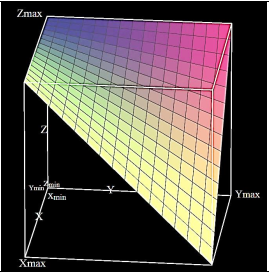
\includegraphics[width=.65\linewidth,]{hw02q5.png}
\end{center}


\newpage
\begin{mybox2}{بخش دوم: مسائل تحلیلی}
با توجه به تعاریف تعادل‌های نش و همبسته، هر یک از مسائل 6 تا 8 را تحلیل کرده و پاسخ مناسبی برای آن بیابید. 
\end{mybox2}

\question
با در نظر داشتن رابطه
 \lr{payoff}
ها در تعادل نش و تعادل همبسته 
\lr{(correlated)}،
 آیا ممکن است تعادل همبسته‌ای وجود داشته باشد که در آن 
 \lr{payoff} 
 هر دو بازیگر کمتر از 
  \lr{payoff}
 آن‌ها در بدترین تعادل نش متقارن (تعادل نشی که در آن 
  \lr{payoff}
 بازیکنان کمتر از بقیه تعادل نش‌های موجود در بازی است)  باشد؟  توضیح دهید.

\question
تعریف 1
را بخوانید و سپس به پرسش‌های داده شده پاسخ دهید:

\begin{definition}{تعادل همبسته نامرغوب}{def1}
     یک توزیع احتمال مثل
    $p(.)$
    روی فضای عمل جمعی بازیگران یک «تعادل همبسته نامرغوب 
    \lr{(CCE)}»\LTRfootnote{Coarse correlated equilibrium}
        نامیده می‌شود هرگاه برای کلیه بازیگران مثل $i$ و برای هر استراتژیِ محض مثل
        $ s^{\prime}_{i} \in S_i $
        از وی داشته باشیم:
        $ U^{\prime}_i(p) \geq  U^{\prime}_i(p; s^{\prime}_{i}) $
        که در آن:
        \begin{equation}\label{eq:1}
               U^{\prime}_i(p; s^{\prime}_{i}) := \sum_{(s_1, ..., s_n) \in S} p(s_1, ..., s_n) u_i(s_1, ..., s_{i-1},  s^{\prime}_i, s_{i+1}, ..., s_n)
        \end{equation}
        
        به تعبیر شهودی مطابق رابطه 
        \ref{eq:1}،
         تحقق
        \lr{CCE} 
        مستلزم این است که «تبعیت از سیگنال پیشنهادیِ داور» (مثلاً $ s_i$) (که ماحصل نمونه برداری از توزیع
        $ p(.)$ 
        است)، پیش از مشاهده‌ی $ s_i $ یک
        \lr{best response}
         باشد. به عبارت دیگر، در این مفهوم تعادلی، هر بازیگر ناگزیر است که از قبل، در خصوص تبعیت/عدم تبعیت از سیگنال‌های داور تعهد بدهد و پس از مشاهده‌ی سیگنال، مجاز به تخطی از تعهد خود نیست. با این ضوابط، 
          $ p(.)$ 
         نمایان‌گر یک 
                \lr{CCE}  
          خواهد بود اگر که هیچ بازیگری (به‌طور یک‌جانبه) انگیزه‌ای برای عدم تعهد به سیگنال‌های داور نداشته باشد.    
\end{definition}
حال، بازی ماتریسی زیر را در نظر بگیرید و نامعادلات مبیّن
 \lr{CE}
 و
 \lr{CCE}
 را از منظر بازیگر سطری (بازیگر 1) بنویسید:
 
 { \centering
     \begin{LTR}
         \begin{tabular}{l|l|l|l}
             \multicolumn{2}{l}{\multirow{2}{*}{}}                                               & \multicolumn{2}{c}{$Column$}                              \\ \cline{3-4} 
             \multicolumn{2}{l}{}                                                                & \multicolumn{1}{|l|}{$a$}    & \multicolumn{1}{l|}{$b$}    \\ \cline{2-4} 
             \multicolumn{1}{c|}{\multirow{2}{*}{$Row$}} & \multicolumn{1}{l|}{$A$} & \multicolumn{1}{l|}{$(0,1)$} & \multicolumn{1}{l|}{$(6,0)$} \\ \cline{2-4} 
             \multicolumn{1}{c|}{}                                     & \multicolumn{1}{l|}{$B$} & \multicolumn{1}{l|}{$(2,0)$} & \multicolumn{1}{l|}{$(5,2)$} \\ \cline{2-4} 
              \multicolumn{1}{c|}{}                                     & \multicolumn{1}{l|}{$C$} & \multicolumn{1}{l|}{$(3,4)$} & \multicolumn{1}{l|}{$(3,3)$} \\ \cline{2-4} 
         \end{tabular}
     \end{LTR}
 }

\question
برای یک بازی ماتریسی دو-نفره، توصیفی از یک برنامه ریاضی ارائه دهید که به کمک آن بتوان تعیین نمود آیا یک پروفایل نش داده شده از نوع بهینه
 \lr{Pareto}
  هست یا خیر.



\newpage
\begin{mybox2}{بخش سوم: مسائل کامپیوتری}
	با استفاده از ابزارهای کامپیوتری مشخص شده و برنامه‌نویسی، مسائل داده شده در این بخش را حل کنید. 
\end{mybox2}

\begin{mybox3}{}

$ \blacktriangleleft$
 بسته‌های نرم‌افزاری مختلفی (تجاری و رایگان)، برای حل مسائل بهینه‌سازی و ارضای محدودیت تحت عنوان کلی 
\lr{Solver}
وجود دارد. این ابزار‌ها ورودی را در قالب یا زبان‌‌های مشخصی از کاربر دریافت کرده، بر اساس آن یک برنامه ریاضی (مدل) تشکیل داده و آن را حل می‌کنند.  
\lr{Solver}های
امروزی با انتشار واسط‌های برنامه‌نویسی کاربردی 
(\lr{API})
برای زبان‌های برنامه‌سازی مختلف، امکانات خود را برای استفاده در ابزارها و برنامه‌های دیگر فراهم کرده‌اند. 
برخی از 
\lr{Solver}های
پرکاربرد و 
\lr{API}
آنها عبارتند از:
 \begin{latin}
    \begin{enumerate}[label*=\arabic*.]
        \item{ 
            \textbf{AMPL} system, C++, C\#, Java, MATLAB, Python, and R callable library (API) 
            \subitem{\href{https://ampl.com/}{https://ampl.com/}}
        }
    
      \item{ 
        \textbf{GUROBI}, C and C++ callable library (API) 
        \subitem{\href{https://www.gurobi.com/documentation/9.0/refman/lp\_format.html}{https://www.gurobi.com/documentation/9.0/refman/lp\_format.html}}
    }

    \item{ 
        \textbf{MATLAB}, the \texttt{intlinprog} function 
        \subitem{\href{ https://www.mathworks.com/help/optim/ug/intlinprog.html}{https://www.mathworks.com/help/optim/ug/intlinprog.html}}
    }

   \item{ 
    \textbf{GAMS} language, C++, .NET, Java, and Python callable library (API)
    \subitem{\href{https://www.gams.com/}{https://www.gams.com/}}
}

     \item{  
        \textbf{Z3}, C++ and Python callable library (API)
        \subitem{\href{https://github.com/Z3Prover/z3}{https://github.com/Z3Prover/z3}}
        \subitem{\href{https://theory.stanford.edu/~nikolaj/programmingz3.html}{https://theory.stanford.edu/~nikolaj/programmingz3.html}}
    }

        \item{
             \textbf{Pulp}, Python callable library (API)
             \subitem{\href{https://coin-or.github.io/pulp/}{https://coin-or.github.io/pulp/}}
            \subitem{\href{http://benalexkeen.com/linear-programming-with-python-and-pulp-part-2/}{http://benalexkeen.com/linear-programming-with-python-and-pulp-part-2/}}
        }
    
      
        \item{ 
            \textbf{GLPK}, C and C++ callable library (API) 
            \subitem{\href{https://www.gnu.org/software/glpk/}{https://www.gnu.org/software/glpk/}}
        }
      \item{ 
        \textbf{ lp\_solve}, C and C++ callable library (API) 
        \subitem{\href{http://lpsolve.sourceforge.net/5.5/}{http://lpsolve.sourceforge.net/5.5/}}
    }
    
        \item{ 
            \textbf{CPLEX}, C, C++ and Java callable library (API) 
            \subitem{\href{https://www.ibm.com/analytics/cplex-optimizer}{https://www.ibm.com/analytics/cplex-optimizer}}
        }
      \item{ 
        \textbf{CBC}, C and C++ callable library (API) 
        \subitem{\href{https://projects.coin-or.org/Cbc}{https://projects.coin-or.org/Cbc}}
    }
    
        \item{ 
            \textbf{MOSEK}, C++, Java, Python and R callable library (API) 
            \subitem{\href{ https://www.mosek.com/}{https://www.mosek.com/}}
        }
     
        \item{ 
           \textbf{SCIP}, C and C++ callable library (API)
            \subitem{\href{https://scip.zib.de/}{https://scip.zib.de/}}
        }
    
       \item{ 
        \textbf{MiniZinc} constraint modeling language
        \subitem{\href{https://www.minizinc.org/index.html}{https://www.minizinc.org/index.html}}
    }
    
        \item{ 
            \textbf{LINGO} optimization modeling software
            \subitem{\href{https://www.lindo.com/index.php/products/lingo-and-optimization-modeling}{https://www.lindo.com/index.php/products/lingo-and-optimization-modeling}}
        }
        
        \item{ 
            \textbf{OpenSolver}, Microsoft Excel plugin
            \subitem{\href{https://opensolver.org/}{https://opensolver.org/}}
        }
        
    \end{enumerate}
 \end{latin}

$ \blacktriangleleft$
در هریک از مسائل زیر، از ابزارهای معرفی شده برای حل برنامه‌های خطی و بهینه‌سازی ‌های حاصله استفاده نمایید. توصیه می‌شود که از ابزارهای رایگان استفاده کنید، زیرا دسترسی به آنها آسان‌تر است. برای نمونه سه ابزار اول، تجاری هستند. همچنین مشابه نبودن ابزار انتخابی شما با دیگران امتیاز مثبت دارد (انتخاب‌های تکراری این امتیاز را از دست می‌دهند). هماهنگی در زمینه انتخاب ابزار بر عهده دانشجویان است. استفاده از ابزاری خارج از این فهرست نیز با ذکر مرجع و توضیحات کافی، بلامانع است. نکات ضروری و مهم در چگونگی استفاده از ابزار ، بایستی در پاسخ شما مستند شود.

\end{mybox3}


\question

یک برنامه کامپیوتری برای محاسبه تعادل همبسته خصوصی
(\lr{private correlated equilibrium})
 در بازی‌های دو نفره متناهی بنویسید. ورودی این برنامه یک فایل حاوی ماتریس 
 \lr{payoff}
 بازیکنان در بازی است. خروجی یک ماتریس هم مرتبه با ماتریس ورودی، محتوی احتمال‌های نسبت‌ داده شد به هر  زوج استراتژی در تعادل، به همراه مقادیر پاداش بازیکنان در تعادل خواهد بود. یک نمونه ورودی و خروجی برای بازی 
 \lr{Shapley}
 (درس 5، اسلاید 5) در زیر داده شده است. بدیهی است که برنامه شما با موارد بیشتری تست می‌شود.
 
\textbf{ ورودی: }
 در سطر اول ابعاد ماتریس ($m\times n$) و در $m$ سطر بعدی، در هر سطر مقادیر 
 \lr{payoff}
 بازیکنان آمده است.
 
 \begin{latin}
     \singlespacing
     \lstinputlisting[language=Python, caption={}, label={code:q11input}]{q11input.txt}
     \doublespacing
 \end{latin}

\textbf{خروجی: }

 \begin{latin}
    \singlespacing
    \lstinputlisting[language=Python, caption={}, label={code:q11output}]{q11output.txt}
    \doublespacing
\end{latin}


\question
یک برنامه کامپیوتری برای محاسبه استراتژی 
\lr{Minimax}
بازیکن سطری در بازی‌های دو نفره مجموع صفر بنویسید. ورودی برنامه ماتریس 
 \lr{payoff}
 بازیکن سطری و خروجی آن بردار احتمال استراتژی 
 \lr{Minimax}
  بازیکن سطری در مقابل ستونی، به همراه مقدار 
  \lr{Minmax value}
  بازیکن سطری است. یک نمونه ورودی و خروجی در زیر داده شده است.

\textbf{ ورودی: }
 در سطر اول ابعاد ماتریس ($m\times n$) و در $m$ سطر بعدی، در هر سطر مقادیر 
\lr{payoff}
بازیکن سطری آمده است.

\begin{latin}
    \singlespacing
    \lstinputlisting[language=Python, caption={}, label={code:q12input}]{q12input.txt}
    \doublespacing
\end{latin}

\textbf{خروجی: }

\begin{latin}
    \singlespacing
    \lstinputlisting[language=Python, caption={}, label={code:q12output}]{q12output.txt}
    \doublespacing
\end{latin}

\end{questions}



%%%%%%%%%%%%%%%%%%%%%%%%
    %%%%  %%%%%%%%%%  %%%%%%
%%%%%%%%%%%%%%%%%%%%%%%%

\newpage
\textbf{تذکرات مهم:}\\
\begin{enumerate}
	\item{
		تمرین‌ها با شماره‌های متوالی 
		(\lr{hw01}
		،
	\lr{hw02}
		و غیره)
		در
	\lr{Edmodo} 
		 قرار می‌گیرند.
}

\item{
	پاسخ تمرین‌ها نیز بایستی در موعد مقرر
	در
	 \lr{Edmodo}  
	بارگذاری شوند. 
	
	\begin{itemize}
		\item{
	برای
	 \textbf{\examnum}~ 
	در موعد 
\textbf{\examdate}~
}
\end{itemize}
}

\item{
	تمرین‌ها بایستی به‌صورت انفــرادی حل شوند. در صورت مشاهده تقلب، نمره منفی به افراد متخلف تعلق می‌گیرد.
}

\item{
	در صورت نیاز، می‌توانید پرسش‌های خود را در \lr{Edmodo} مطرح کنید.
	
	{\flushleft{موفق باشید:)}}
	%برای ارتباط با کمک مدرس‌ها می‌توانید از ایمیل‌های 
	%\href{mailto:m-zakeri@live.com}{\lr{m-zakeri@live.com}} 
%	و%
	%\href{mailto:arman.sanahmadi@gmail.com}{\lr{arman.sanahmadi@gmail.com}} 
	% استفاده کنید. 
}

\end{enumerate}

\vspace{3cm}
\begin{center}
		\drawsnowflake[scale=0.256]{type=A, l-system={order=6,axiom=---fff+++F}, line width=0.16mm}
\end{center}

\end{document}